\chapter{Flashing the FPGAs and CPLDs in the MEGA65}
#
\section{Flashing the Artix 100T main FPGA with VIVADO}

WARNING: Your warranty is now void! Re-programming the MEGA65 FPGA can potentially cause
damage, or leave your MEGA65 in an unresponsive state from which it is very difficult to
recover, i.e., ``bricked''.  Therefore if you choose to open your MEGA65 and reprogram
any of the FPGAs it contains, it is no longer possible to guarantee its correct operation.
Therefore in this case we can not reasonably honour the warranty of the device as a computer.

If you choose to proceed, you will need a TE0790-03 JTAG programming module, a functioning
installation of Xilinx's Vivado software.  This can be done on either Windows or Linux, but
in both cases you will need to install any necessary USB drivers.

XXX - Image of TE0790 fitted in correct place, with jumpers correctly set.

Connect your non-8-bit computer to the FPGA programming device using a mini-USB cable. Open VIVADO, which can be downloaded from the internets.

\begin{figure}
  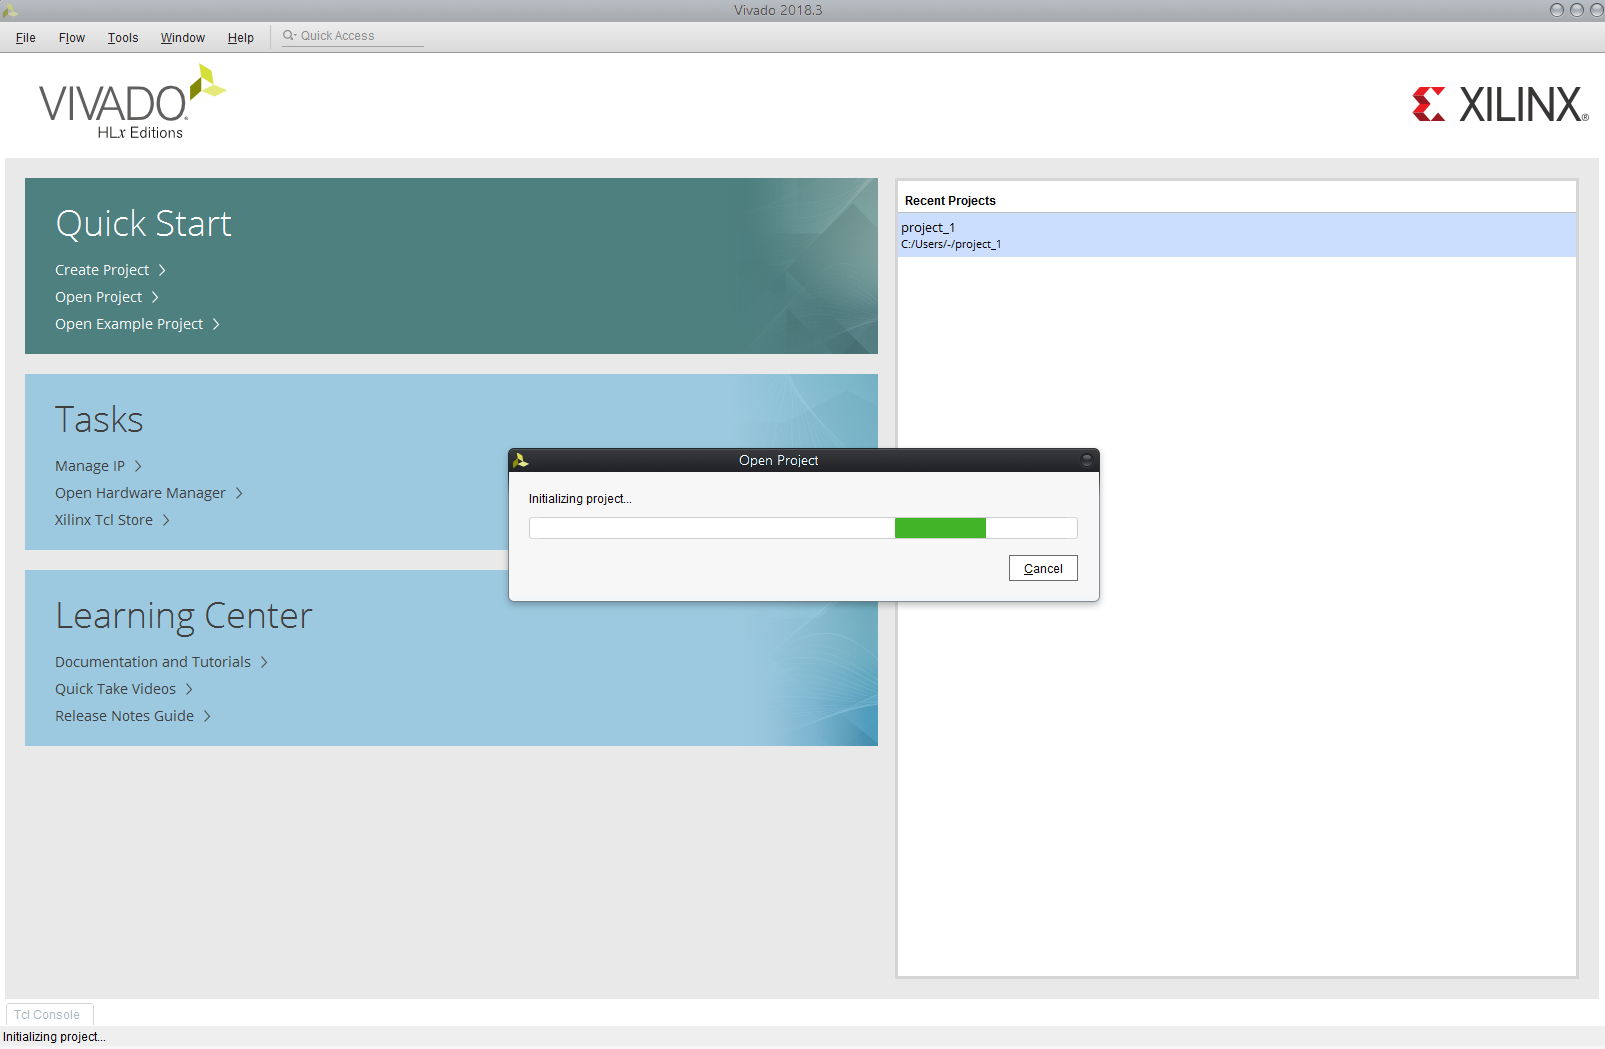
\includegraphics[width=\linewidth]{images/vivado01.png}
  \caption{Step 1: Open a project in VIVADO}
  \label{fig:vivado01}
\end{figure}

To access the Hardware Manager, open a project in VIVADO or create an empty one, if you do not have any projects yet.

\begin{figure}
  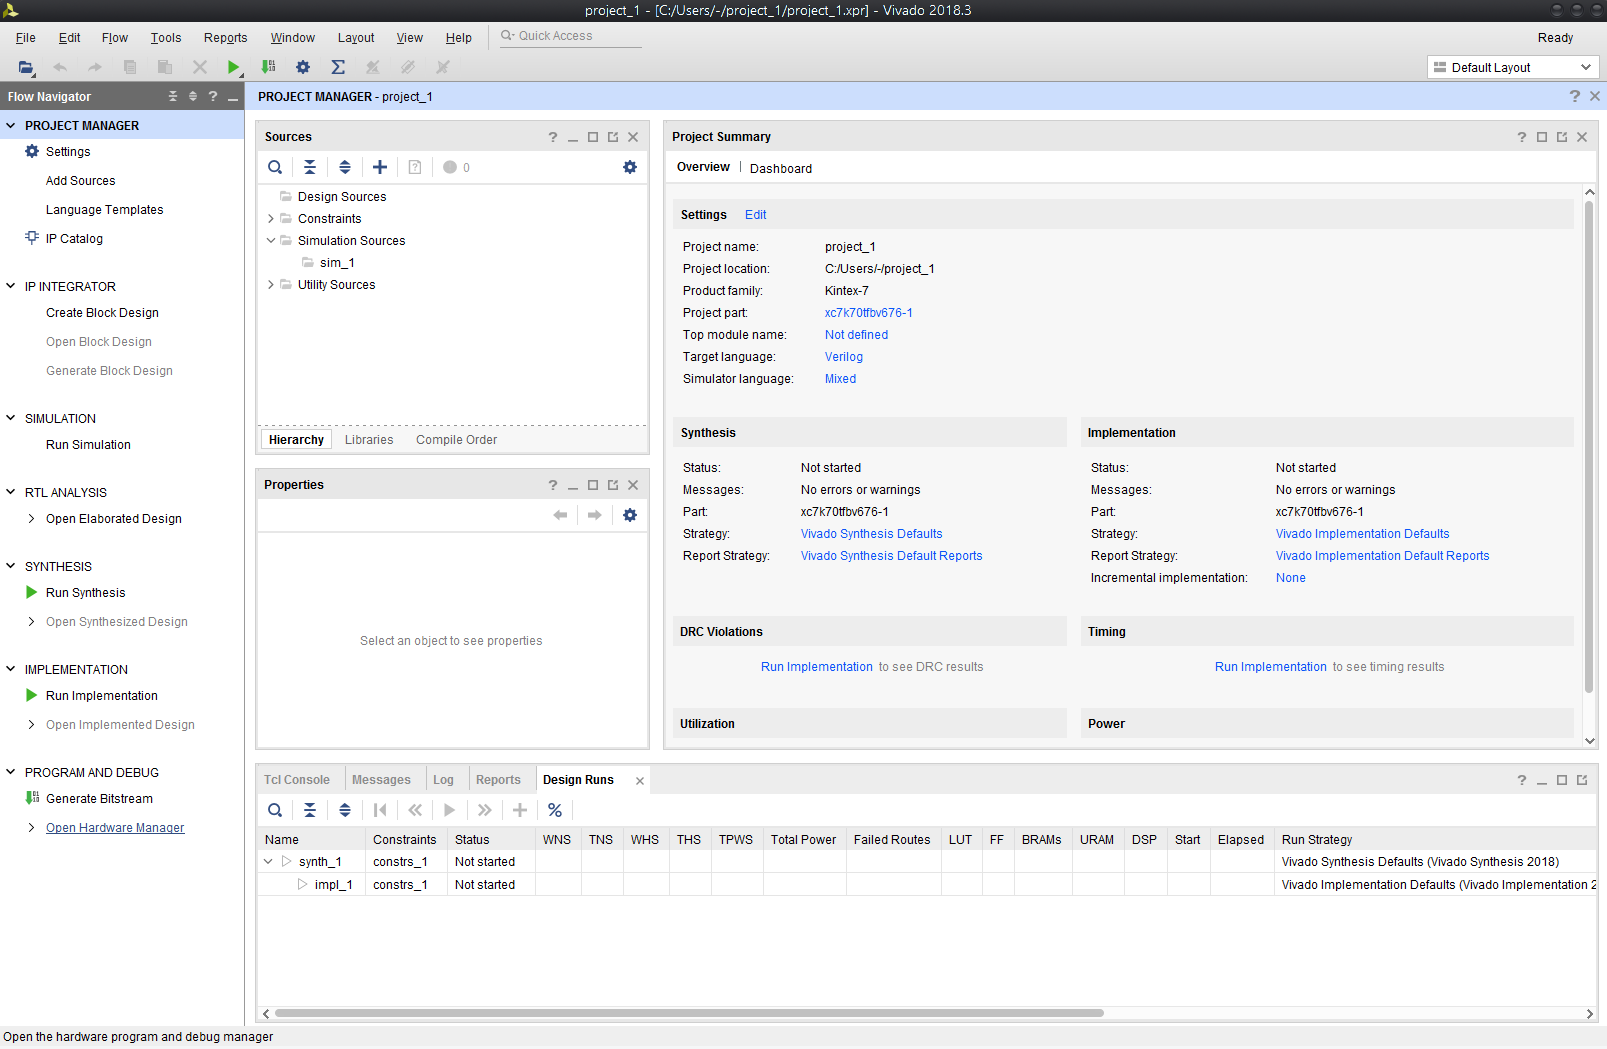
\includegraphics[width=\linewidth]{images/vivado02.png}
  \caption{Step 2: Open Hardware Manager}
  \label{fig:vivado02}
\end{figure}

In the left column, select "Open Hardware Manager" at the very bottom.

\begin{figure}
  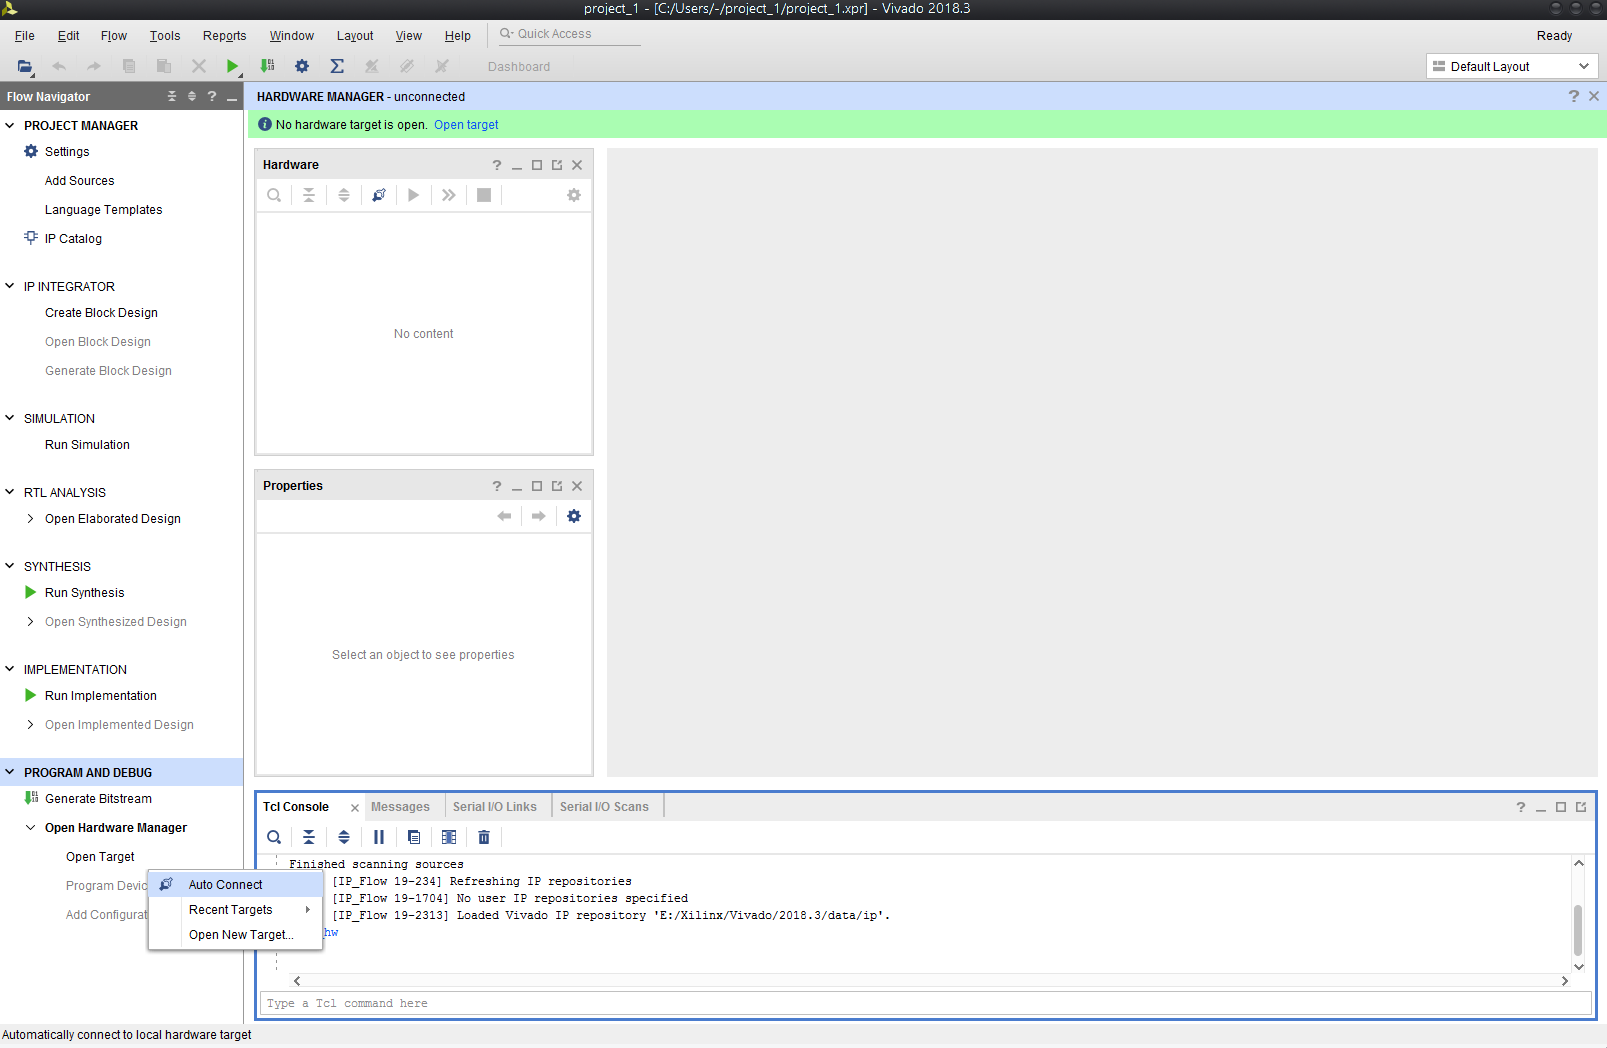
\includegraphics[width=\linewidth]{images/vivado03.png}
  \caption{Step 3: Connect to FPGA}
  \label{fig:vivado03}
\end{figure}

Under "Hardware Manager", choose "Open Target", then "Auto Connect".

\begin{figure}
  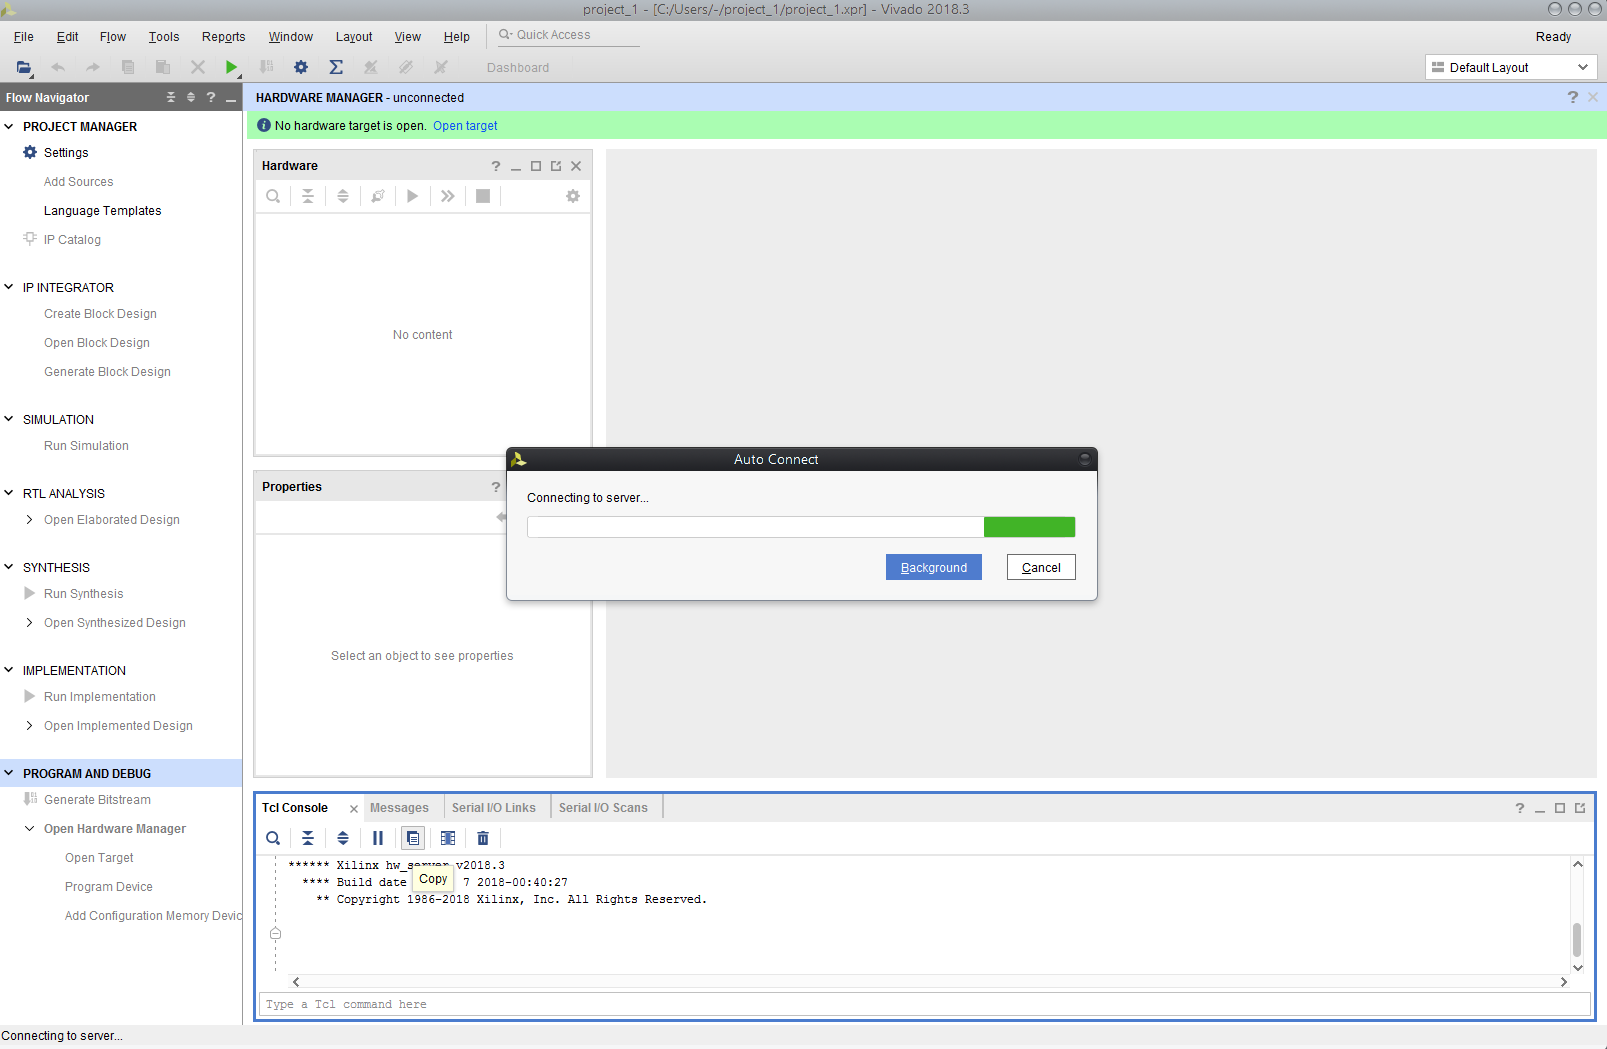
\includegraphics[width=\linewidth]{images/vivado04.png}
  \caption{Step 4: Wait a moment}
  \label{fig:vivado04}
\end{figure}

Wait a moment, "Connecting to server..."  should automatically close without dropping an error to the console.

\begin{figure}
  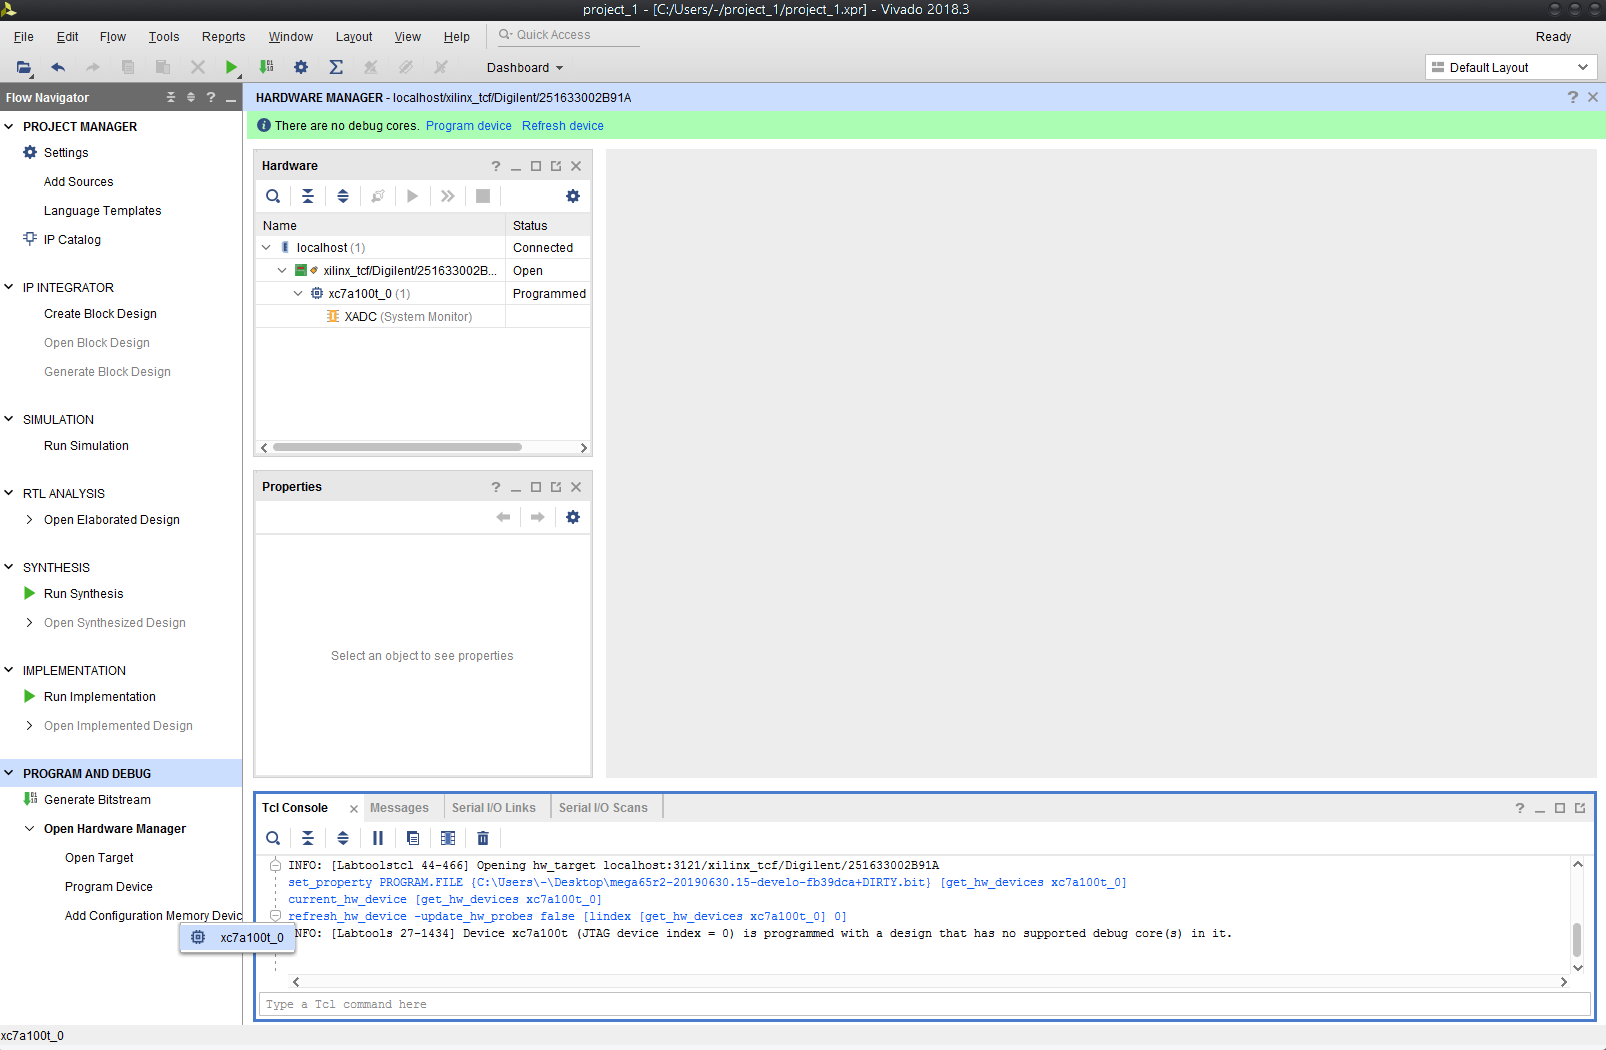
\includegraphics[width=\linewidth]{images/vivado05.png}
  \caption{Step 5: Add Configuration Memory Device}
  \label{fig:vivado05}
\end{figure}

Under "Hardware Manager", choose "Add Configuration Memory Device", then "xc7a100t_0".

\begin{figure}
  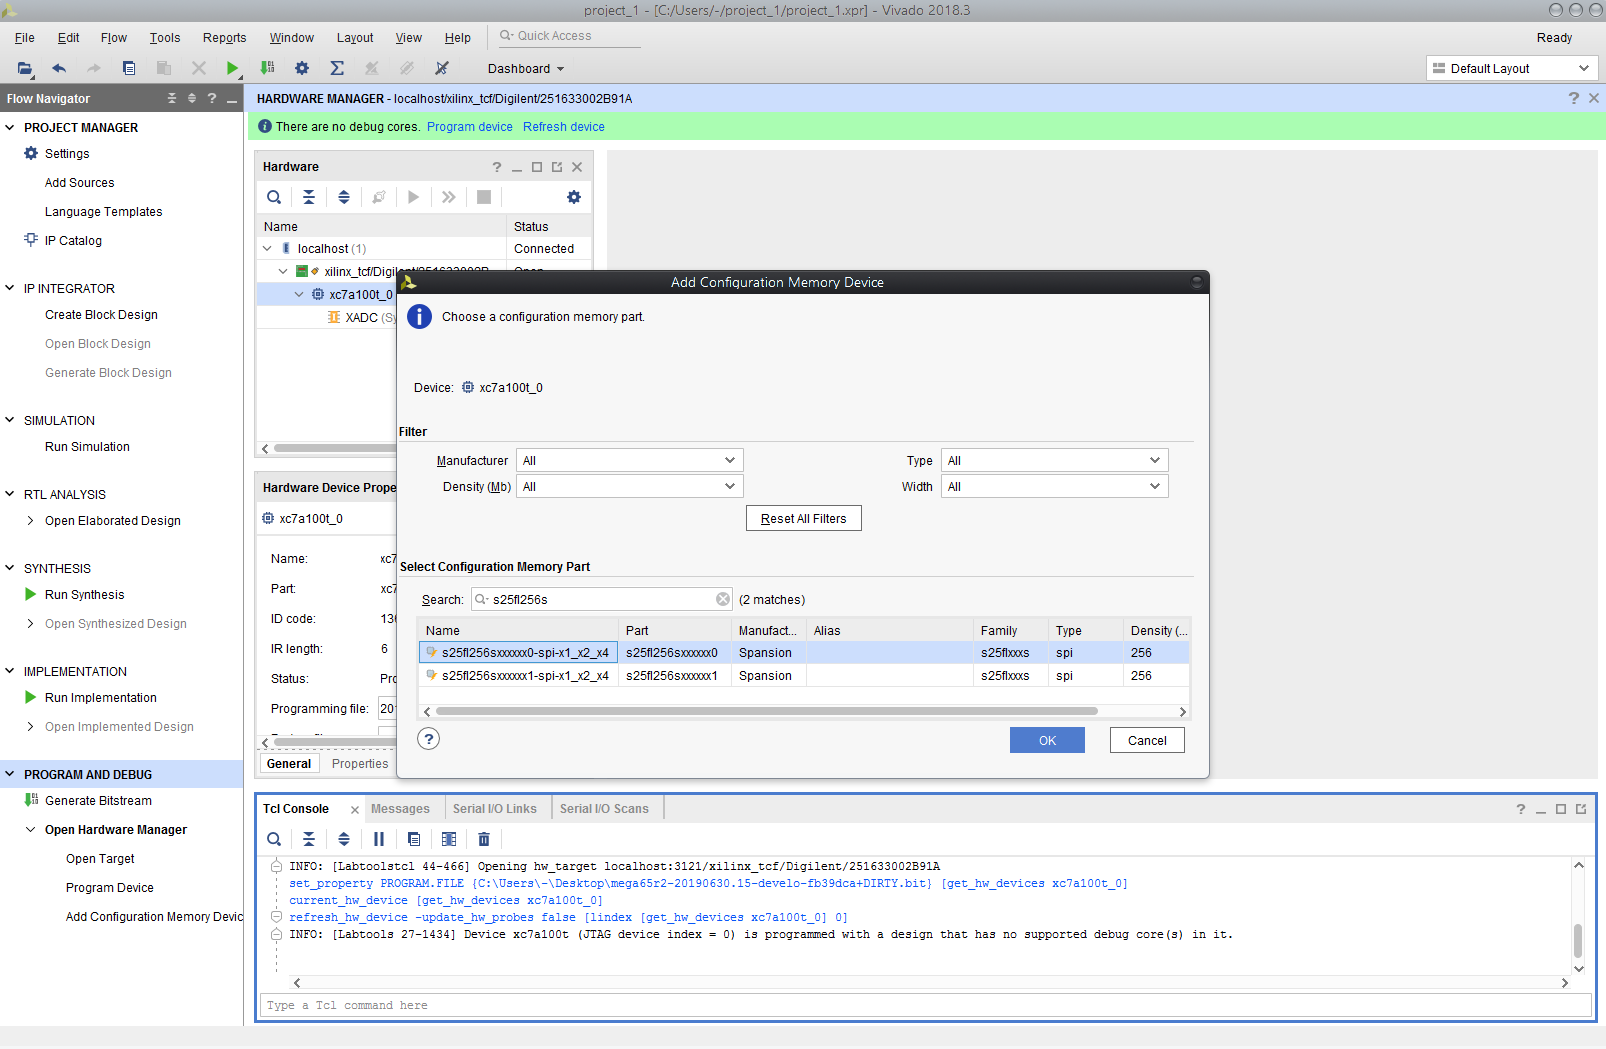
\includegraphics[width=\linewidth]{images/vivado06.png}
  \caption{Step 6: Select Memory Part}
  \label{fig:vivado06}
\end{figure}

In the newly opened dialogue, type "S25fl256s" (without quotes), then select "s25fl256sxxxxxxx0-spi-x1_x2_x4" (the upper one) and click "OK".

\begin{figure}
  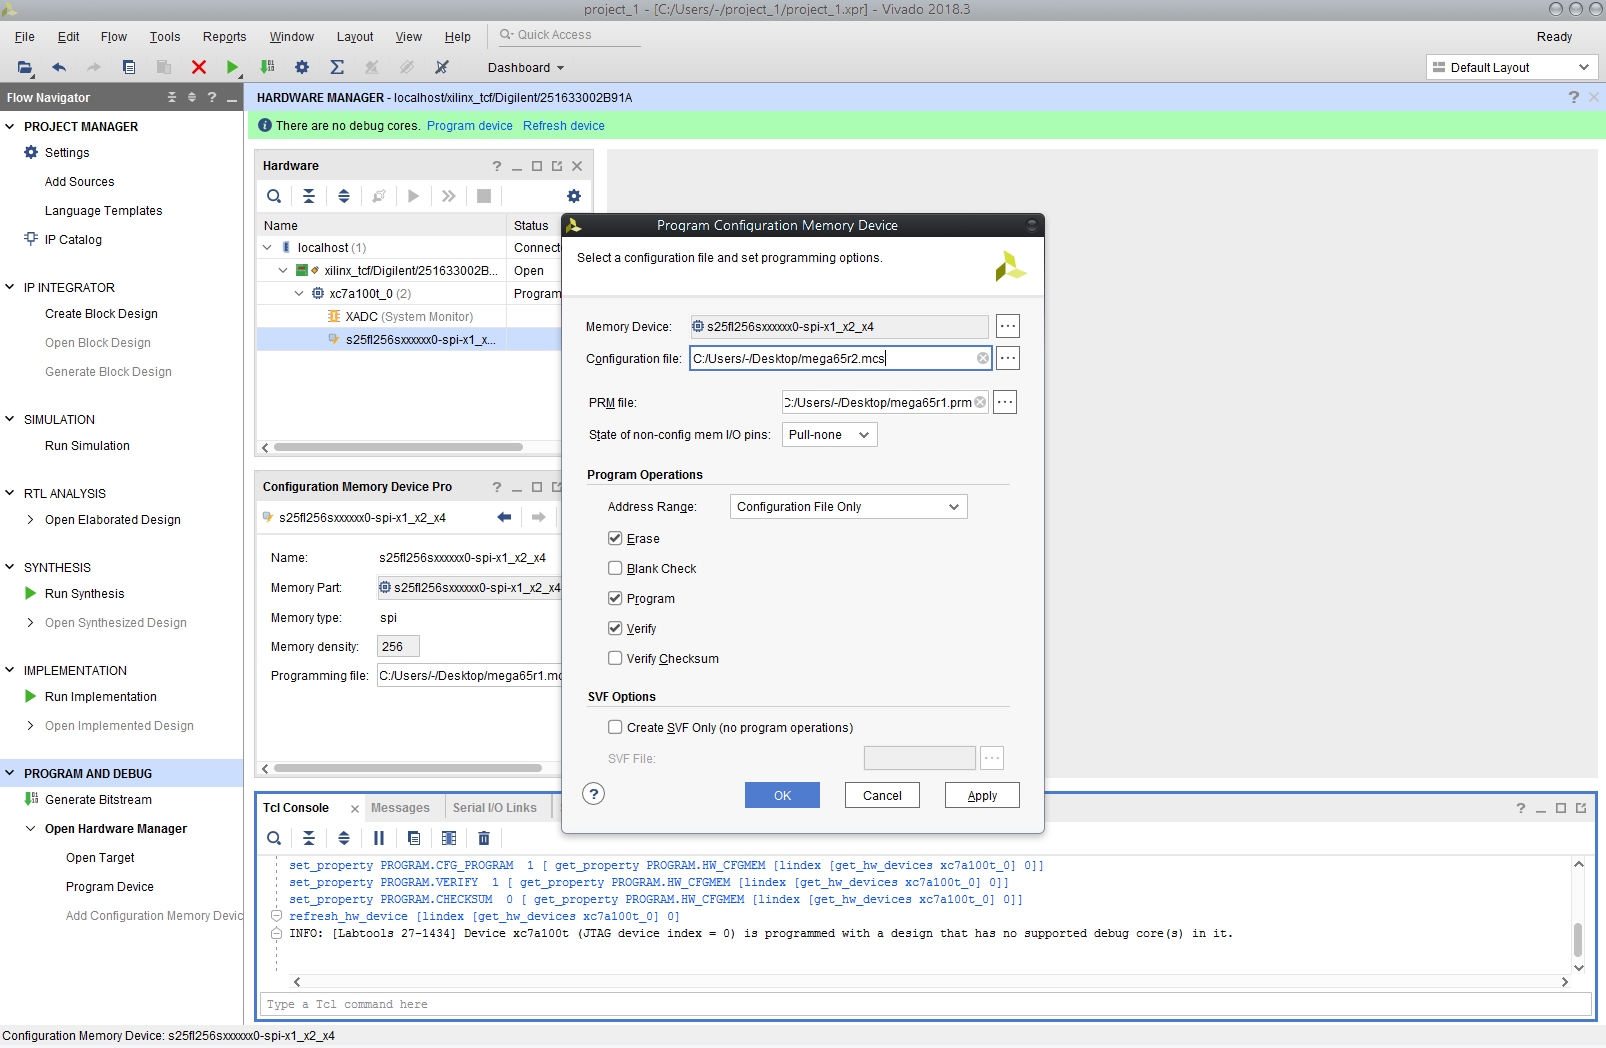
\includegraphics[width=\linewidth]{images/vivado07.png}
  \caption{Step 7: Set programming options}
  \label{fig:vivado07}
\end{figure}

In the next dialogue, choose your local Configuration file, namely a bitstream with file suffix ".mcs". Leave all other parameters as they are (see /ref{fig:vivado07}).

\begin{figure}
  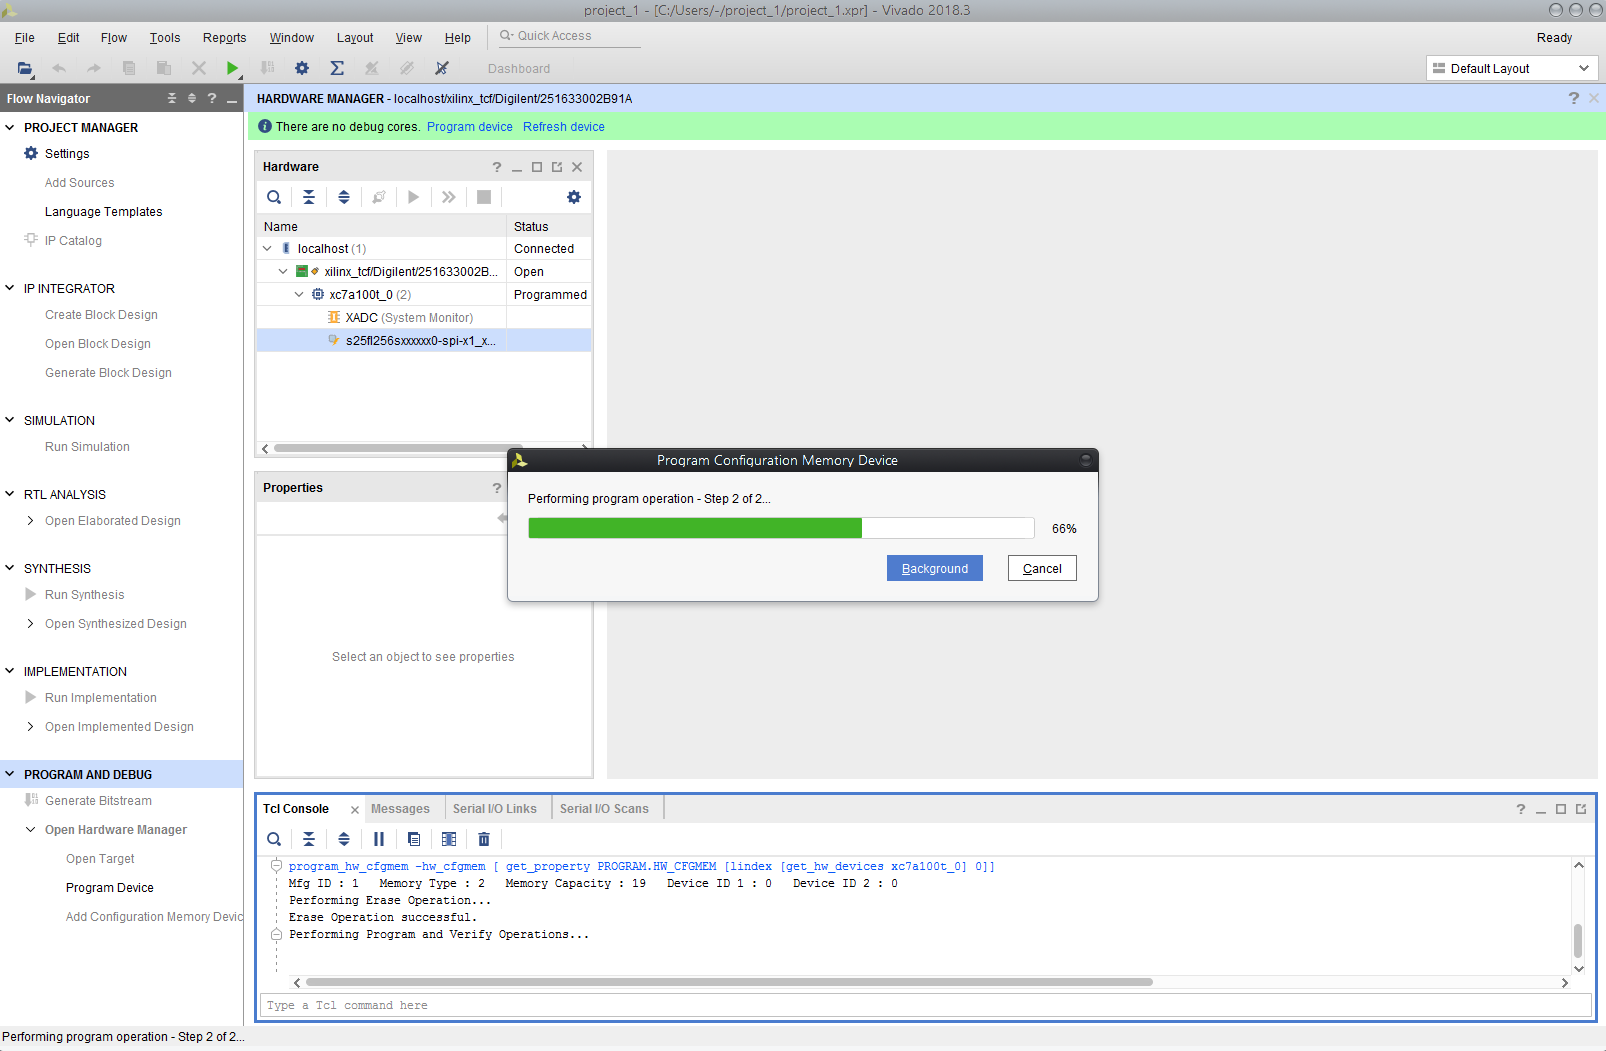
\includegraphics[width=\linewidth]{images/vivado08.png}
  \caption{Step 8: Programming in progress}
  \label{fig:vivado08}
\end{figure}

Patiently wait for the programming to finish, fingers crossed.

\begin{figure}
  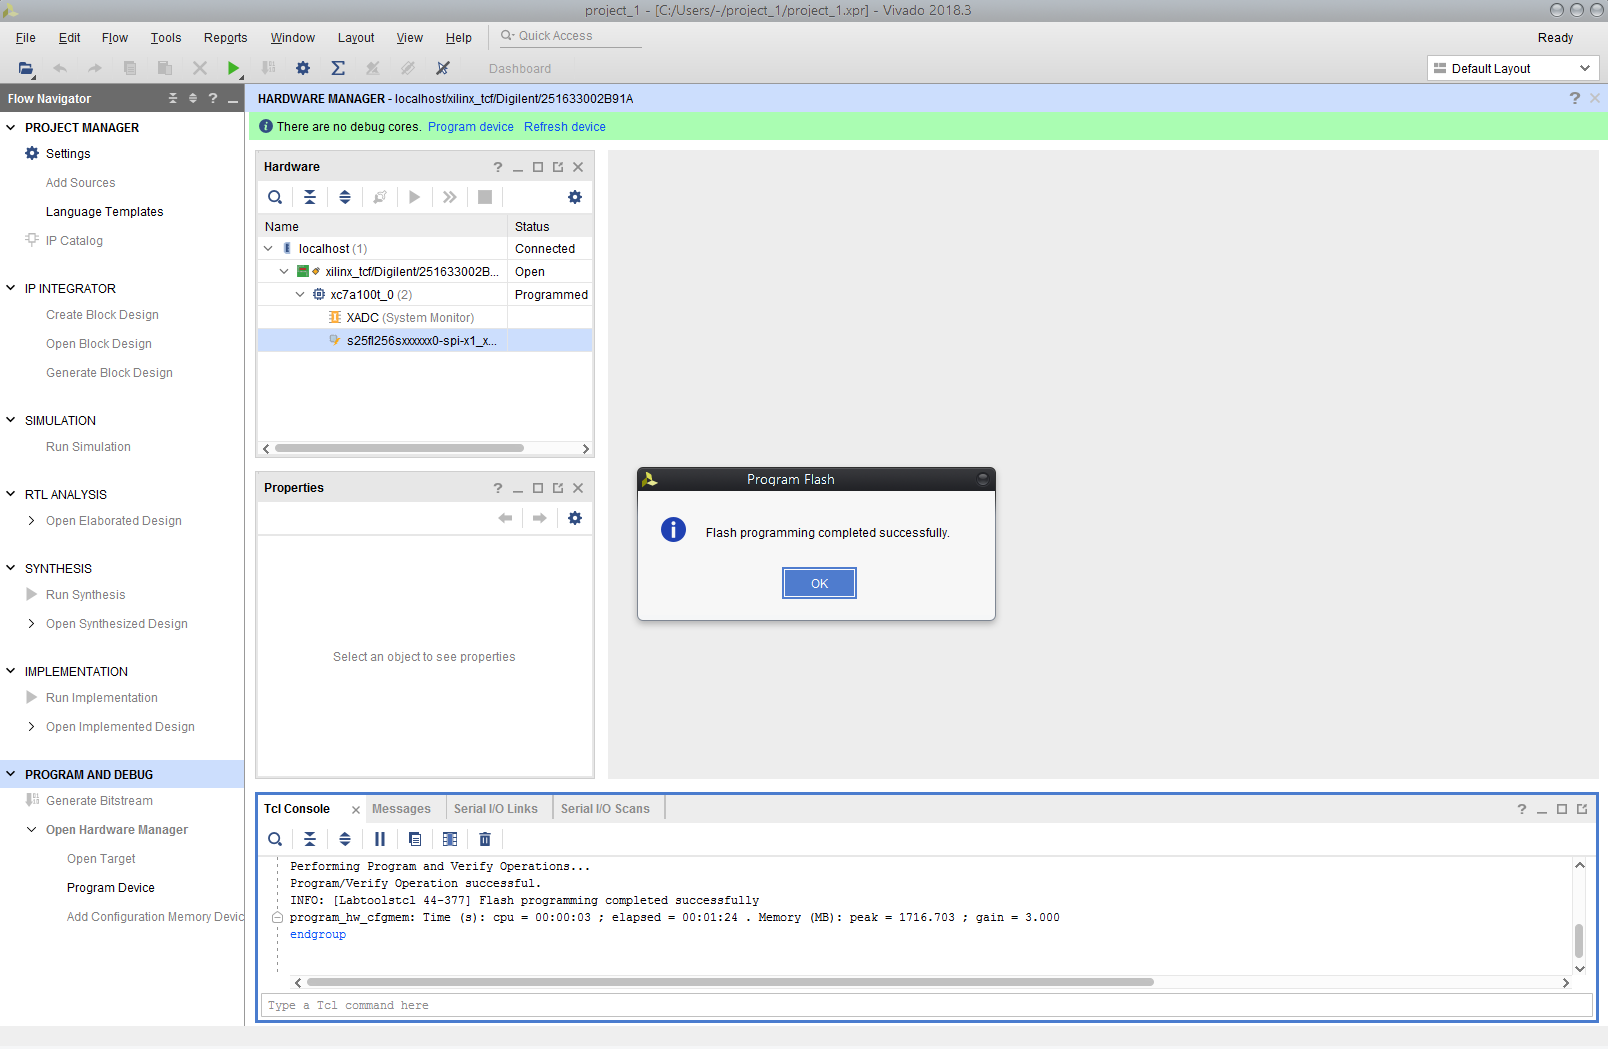
\includegraphics[width=\linewidth]{images/vivado09.png}
  \caption{Step 9: Programming successful}
  \label{fig:vivado09}
\end{figure}

If your screen looks like /ref{fig:vivado09}, your new bistream has been successfully flashed into the Artix 100T FPGA!

\begin{figure}
  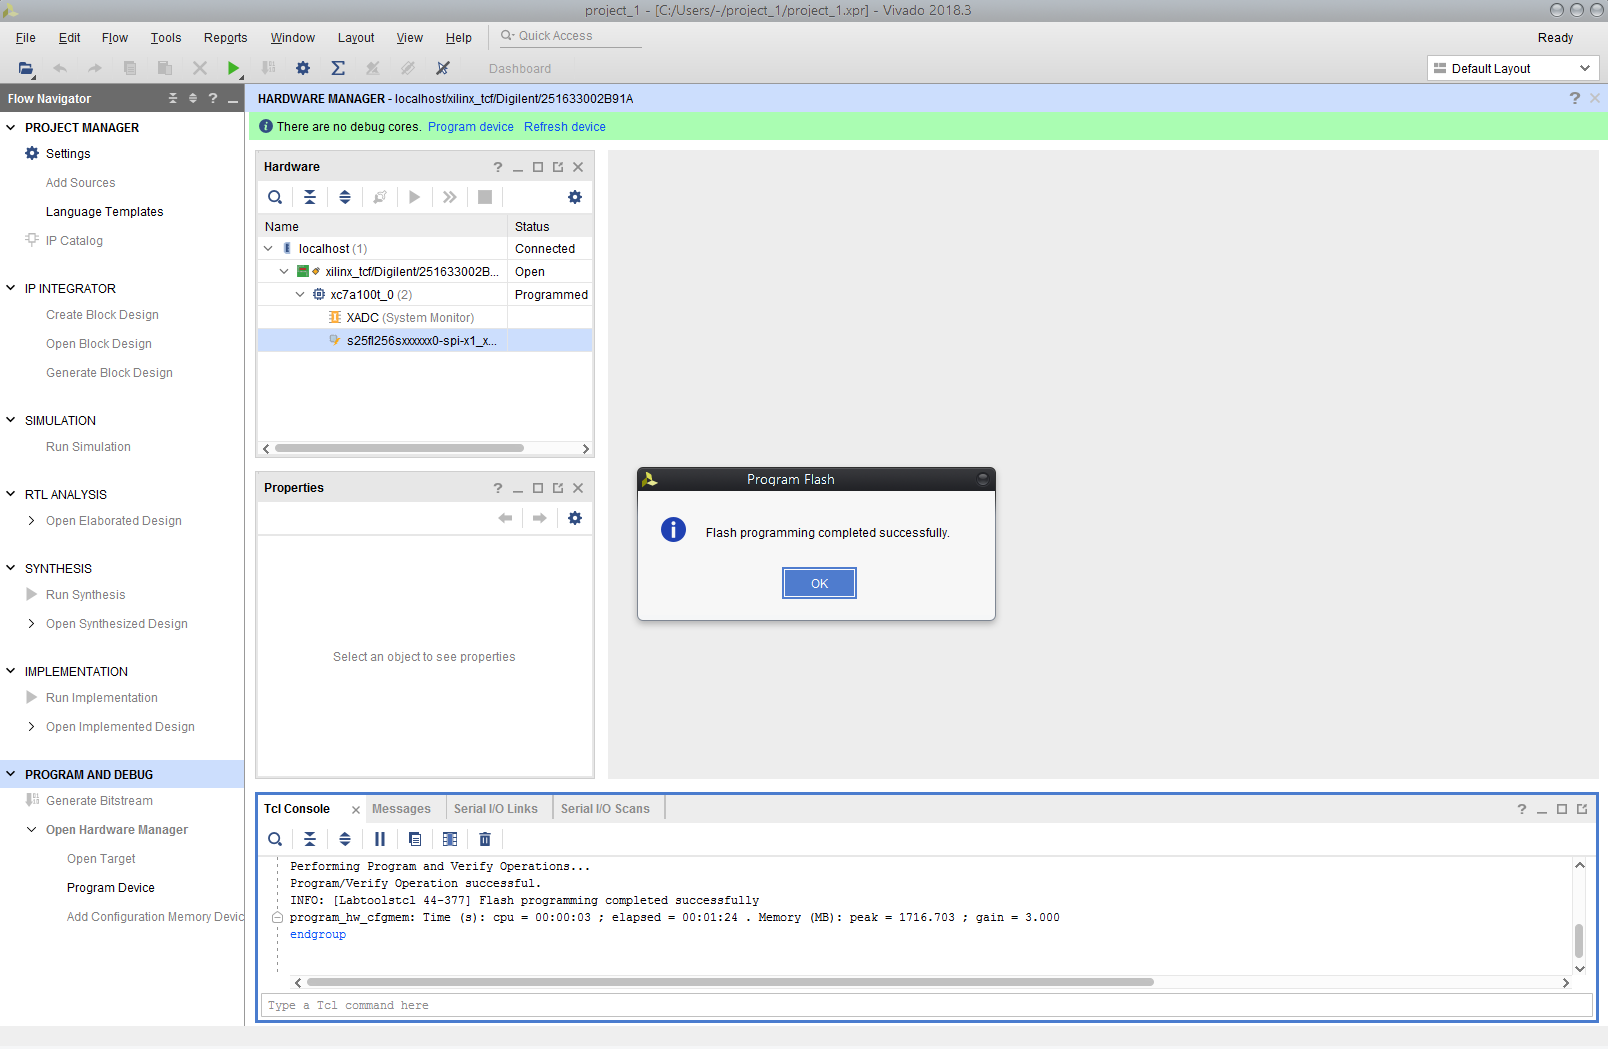
\includegraphics[width=\linewidth]{images/vivado09.png}
  \caption{Step 10: Reflashing the FPGA}
  \label{fig:vivado10}
\end{figure}

If you want to repeat the process, you might find the "Add Configuration Memory Device" option in step 5 greyed out. Instead, select "s25fl256sxxxxxxx0-spi-x1_x2_x4"  in the "Hardware" window, press right mouse button and select "Program Configuration Memory Device" to flash.
















